
\subsection{Technology Overview}
MMEA platform is designed to use Service Oriented Architecture (SOA) which means that different processes and components are implemented as independent and flexible services. These loosely coupled services use one another through open interfaces. This architecture pattern facilitates the integration of new components into the system and allows the services to be distributed into several physical machines. 

The MMEA platform runs on the Amazon Web Services (AWS) cloud which consists of Amazon Elastic Compute Cloud (EC2) and Amazon Simple Storage Service (S3). The former is a cloud computing platform where users can install virtual servers called instances and the latter is a cloud storage service where users can store application data through web services. Both services are billed as a pay-as-you-go service which means that users can scale the computing resources whenever needed and pay only for the resources used. By using a cloud-based approach the costs and the amount of maintenance of physical servers can be eliminated.

The SOA principle in MMEA is implemented using an open-source Enterprise Service Bus (ESB) from WSO2 software company. WSO2 ESB is a lightweight and high performance integration layer between different services. It uses Java Message Service (JMS) for exchanging messages between distributed and loosely-coupled services. The ESB integrates the five other MMEA layers
\begin{description}
\item[Sensor Layer]{Connects to sensor systems with sensor-specific adapters}
\item[Storage Layer]{Stores data into a database and loads data from it}
\item[Model Layer]{Runs computations based on problem-specific models}
\item[Control Layer]{Provides interfaces for monitoring and managing the system}
\item[Presentation Layer]{Provides data for external applications}
\end{description}
These layers are shown in Figure~\ref{fig:mmea}.

\begin{figure}[here]
\centering
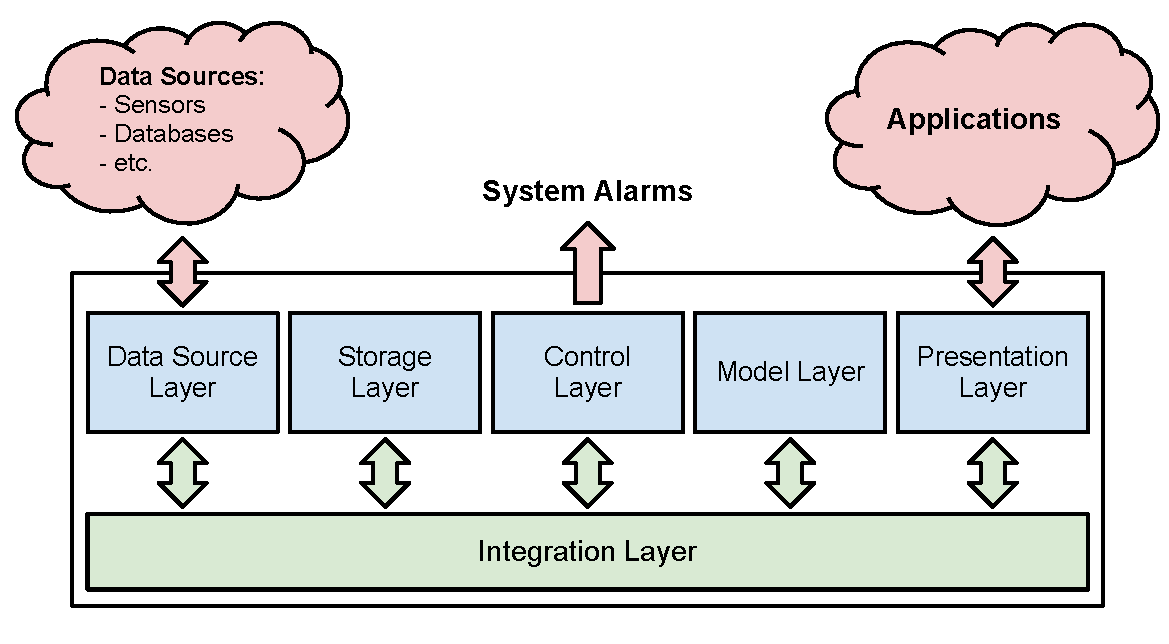
\includegraphics[scale=0.7]{images/mmea.pdf}
\caption{MMEA Platform layers.}
\label{fig:mmea}
\end{figure}

At the core of the application layer there is a component called publish/subscribe which works over SOAP, an XML-based web service for messaging. External applications can publish their data feed and send their new data into the MMEA platform. Other parties can subscribe to these feeds and utilize the data in their processes, such as alarm services.

The MMEA platform has its own data format called MMEA Bus Message, which is an XML-based message format. It has a separate XML schema for common platform messages, sensor observation messages, forecast messages and complex event messages. For example, a sensor observation message contains information about the producer and the location of the sensor, as well as the measurand and the observed value. The sensor layer adapters define XSLT (Extensible Stylesheet Language Transformations) transformations from the producers' data formats into the MMEA Message Bus format.



\subsection{Integrating the Predictive Component}
The predictive complex event processing network must be integrated to the existing platform architecture so that the platform remains easily maintainable. As can be seen from the layer descriptions in the previous chapter, the MMEA platform has a model layer, which is used to run computations on problem-specific models. The predictive component can be integrated to this layer and run on the same physical computational cluster.

Another, and perhaps a better way to integrate the predictive component is to create an external application that is loosely coupled with the MMEA platform. In this approach the CEP engine and the predictive component are running on separate machine and use the publish/subscribe method provided by MMEA platform. Predictive component subscribes to feed that provides new sensor data. Then, having analyzed the data, it can publish the complex events, that is, the alarms back to the MMEA platform.




